\documentclass[aspectratio=169]{beamer}

\usetheme{metropolis}

% ENCODING AND LANGUAGE
\usepackage[english]{babel}

\usepackage[utf8]{inputenc}     % Universal encoding
\usepackage[T1]{fontenc}        % Font encoding

% FONT
\usepackage{courier}            % Courier as \ttdefault
% \usepackage{psfrag}             % replace PostScript fonts

% OTHER HELPERS AND SETTINGS
% \usepackage{graphicx}           % Include graphics to document
% \usepackage{amsmath,amssymb,amstext}  % support for mathematics ttt

% \usepackage{listings}           % code listings
% \lstset{basicstyle=\footnotesize\ttfamily,breaklines=true}

% \usepackage{units}
\usepackage{siunitx}            % SI-Unit support

% TITLE PAGE SETTINGS
\title{Angel Introduction: Camera and Video Mixer}
% \date{\today \currenttime}
\author{jtbx (he/him)}
\institute{C3VOC
	\begin{flushright}
		\includegraphics[height=0.4\textheight]{images/qr-code.png}\\
		https://github.com/voc/engelschulung
	\end{flushright}
}

%% START OF DOCUMENT
\begin{document}
\maketitle

\begin{frame}{New Introduction Meeting Format}
	\begin{itemize}
		\item We're trying a new way to do this introduction meeting!
		\item Less frontal lessons, more hands-on for new people
		\item Prioritize experienced angels to ensure quality
		\item Downside: We will limit the number of angels
		\begin{itemize}
			\item This way you have more chances to improve your skills
			\item Goal: Everybody should be able to do at least 2 shifts per day
			\item We need to try, how many angels we actually need
		\end{itemize}
	\end{itemize}
\end{frame}

% !TEX root = ../main.tex

\begin{frame}{General}
	\begin{itemize}
		\item We will stream, record and publish nearly all talks with your help
		\item You can operate the cameras and video mixer
		\item At do-not-record talks we also need angels % for guarding the camera or to do a recording, but no live stream
		\item We (people from c3voc) will be there to help
		\item The live stream video signal will also be the final recording
		\item We aim for consistent quality, but everybody make mistakes -- don't blame yourself!
	\end{itemize}
\end{frame}



\section{Recap: Audio Hardware}
% !TEX root = ../main.tex

\begin{frame}{Audio Mixer Controls: Levels}
	\begin{columns}[T,onlytextwidth]
		\column{0.6\textwidth}
		\begin{figure} 
			\centering
			\includegraphics[width=0.9\textwidth]{images/touchmix-main-controls.jpg}
			\caption{Touchmix Main Controls}
		\end{figure}
		\column{0.4\textwidth}
		\begin{itemize}
			\item Mute unused microphones (bottom row)
			\item Adjust hall loudness with rightmost fader
			\item Adjust individual microphone level with fader or reduce "trim" knob when it's clipping
			\item Please keep microphones un-muted during applause
		\end{itemize}
	\end{columns}
\end{frame}

\begin{frame}{Audio Mixer Controls: Second Page}
	\begin{columns}[T,onlytextwidth]
		\column{0.6\textwidth}
		\begin{figure} 
			\centering
			\includegraphics[width=0.9\textwidth]{images/touchmix-cam-controls.jpeg}
			\caption{Touchmix Second Page}
		\end{figure}
		\column{0.4\textwidth}
		\begin{itemize}
			\item If mute buttons are yellow, go back to "Main Mix" page
			\item If anything else is shown, just press "Home" button
		\end{itemize}
	\end{columns}
\end{frame}

\begin{frame}{Audio Mixer Controls: Headphones}
	\begin{columns}[T,onlytextwidth]
		\column{0.6\textwidth}
		\begin{figure} 
			\centering
			\includegraphics[width=0.9\textwidth]{images/touchmix-cam-headphones.jpg}
			\caption{Touchmix Headphones}
		\end{figure}
		\column{0.4\textwidth}
		\begin{itemize}
			\item Press "Phones" to adjust headphone loudness
			\item "Cue" on Camera/ Recoding mix must be selected
			\item Rotary knob can be used to adjust selected parameter (headphone level, channel level, etc.)
		\end{itemize}
	\end{columns}
\end{frame}

% !TEX root = ../main.tex

\begin{frame}{Microphones}
	\begin{itemize}
		\item We prefer headset microphones over handheld for speakers
		\item Distance to mouth will be constant -> more consistent audio level
		\item Handheld microphones for heralds and Q\&A
		\item Our transmitters also have a mute button (yellow light = muted)
		\item Please check battery level from time to time
	\end{itemize}
\end{frame}

\begin{frame}{Headset Placement}
	\begin{columns}[T,onlytextwidth]
		\column{0.6\textwidth}
		\begin{figure} 
			\centering
			\includegraphics[width=0.9\textwidth]{images/headset-side.jpeg}
			\caption{Good headset microphone placement}
		\end{figure}
		\column{0.4\textwidth}
		\begin{itemize}
			\item Microphone shall be at the corner of the mouth
			\item Boom can slide back and forth
			\item If too far in front, there will be too much wind noise
			\item Distance to face: About 2 cm
			\item Bend boom carefully
		\end{itemize}
	\end{columns}
\end{frame}



\section{New Features and Setup Specialities}
% !TEX root = ../main.tex

\begin{frame}{New Voctomix Features}
	\begin{itemize}
		\item Voctomix has presets now!
		\begin{itemize}
			\item Lecture mode with slides and camera on one button!
			\item No more accidents with the slides in small picture
		\end{itemize}
		\item Use lecture mode more often
	\end{itemize}
\end{frame}

\begin{frame}{New Voctomix Features}
	\begin{figure}
		\centering
		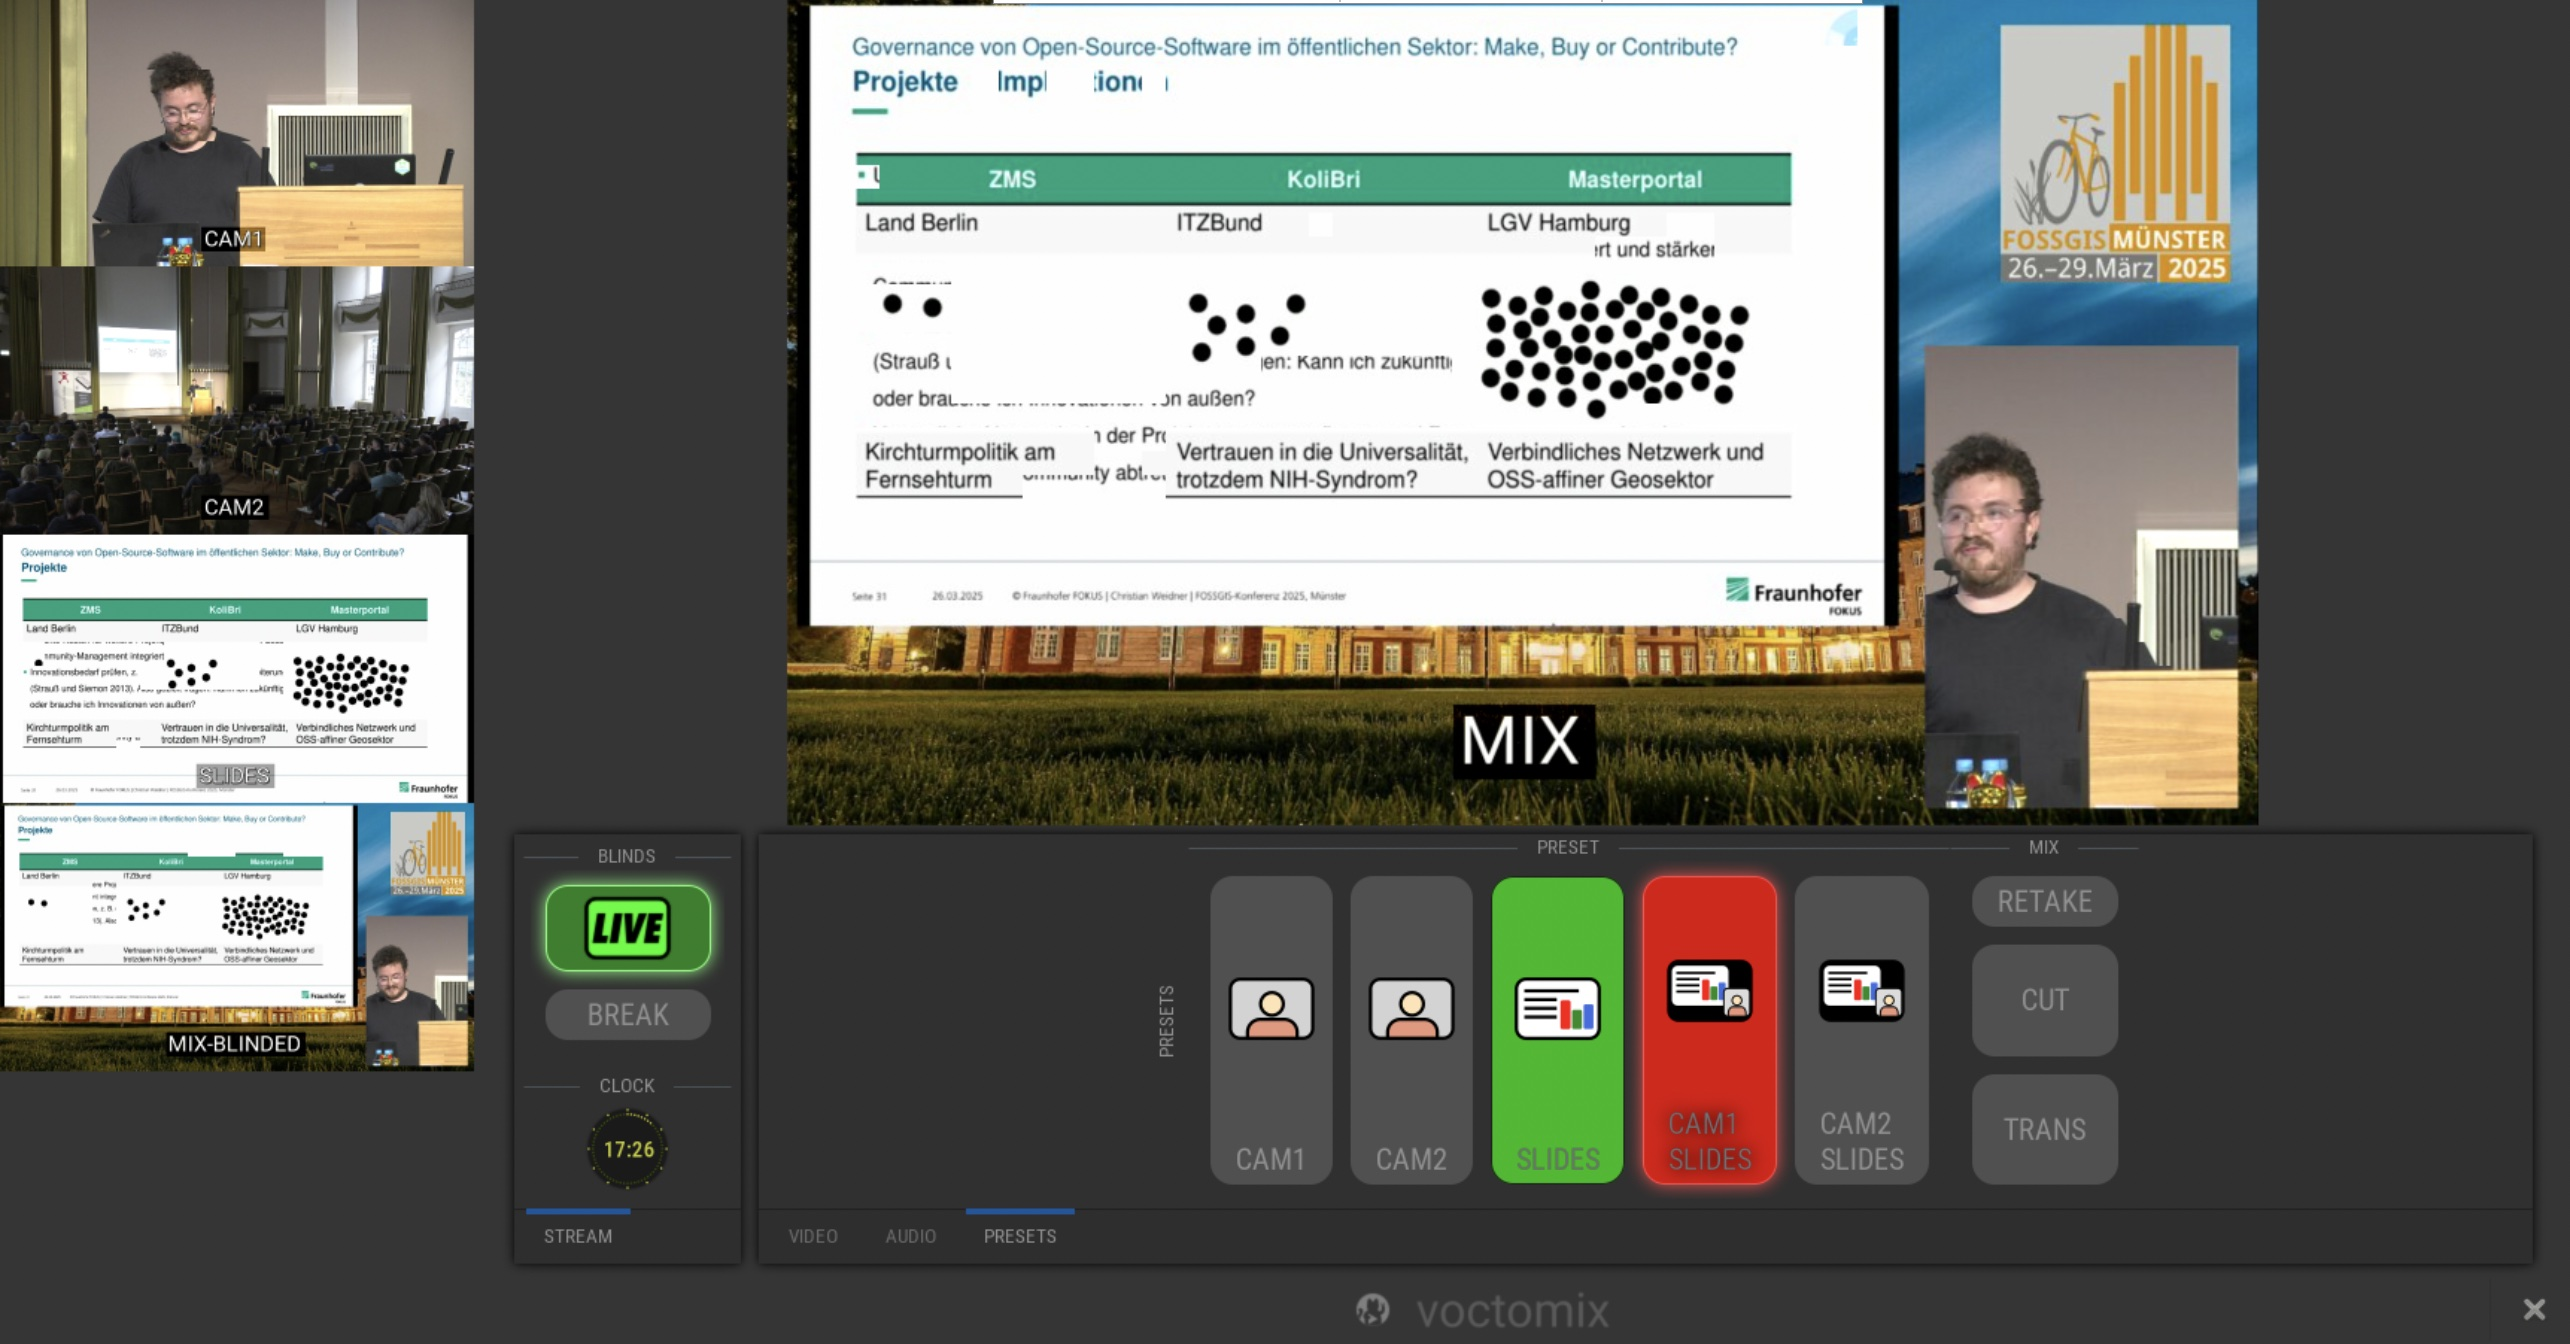
\includegraphics[width=0.9\textwidth]{images/voctomix2-presets-lecture.jpg}
		\caption{Voctomix2 Presets: Lecture Mode}
	\end{figure}
\end{frame}

\begin{frame}{New Voctomix Features}
	\begin{figure}
		\centering
		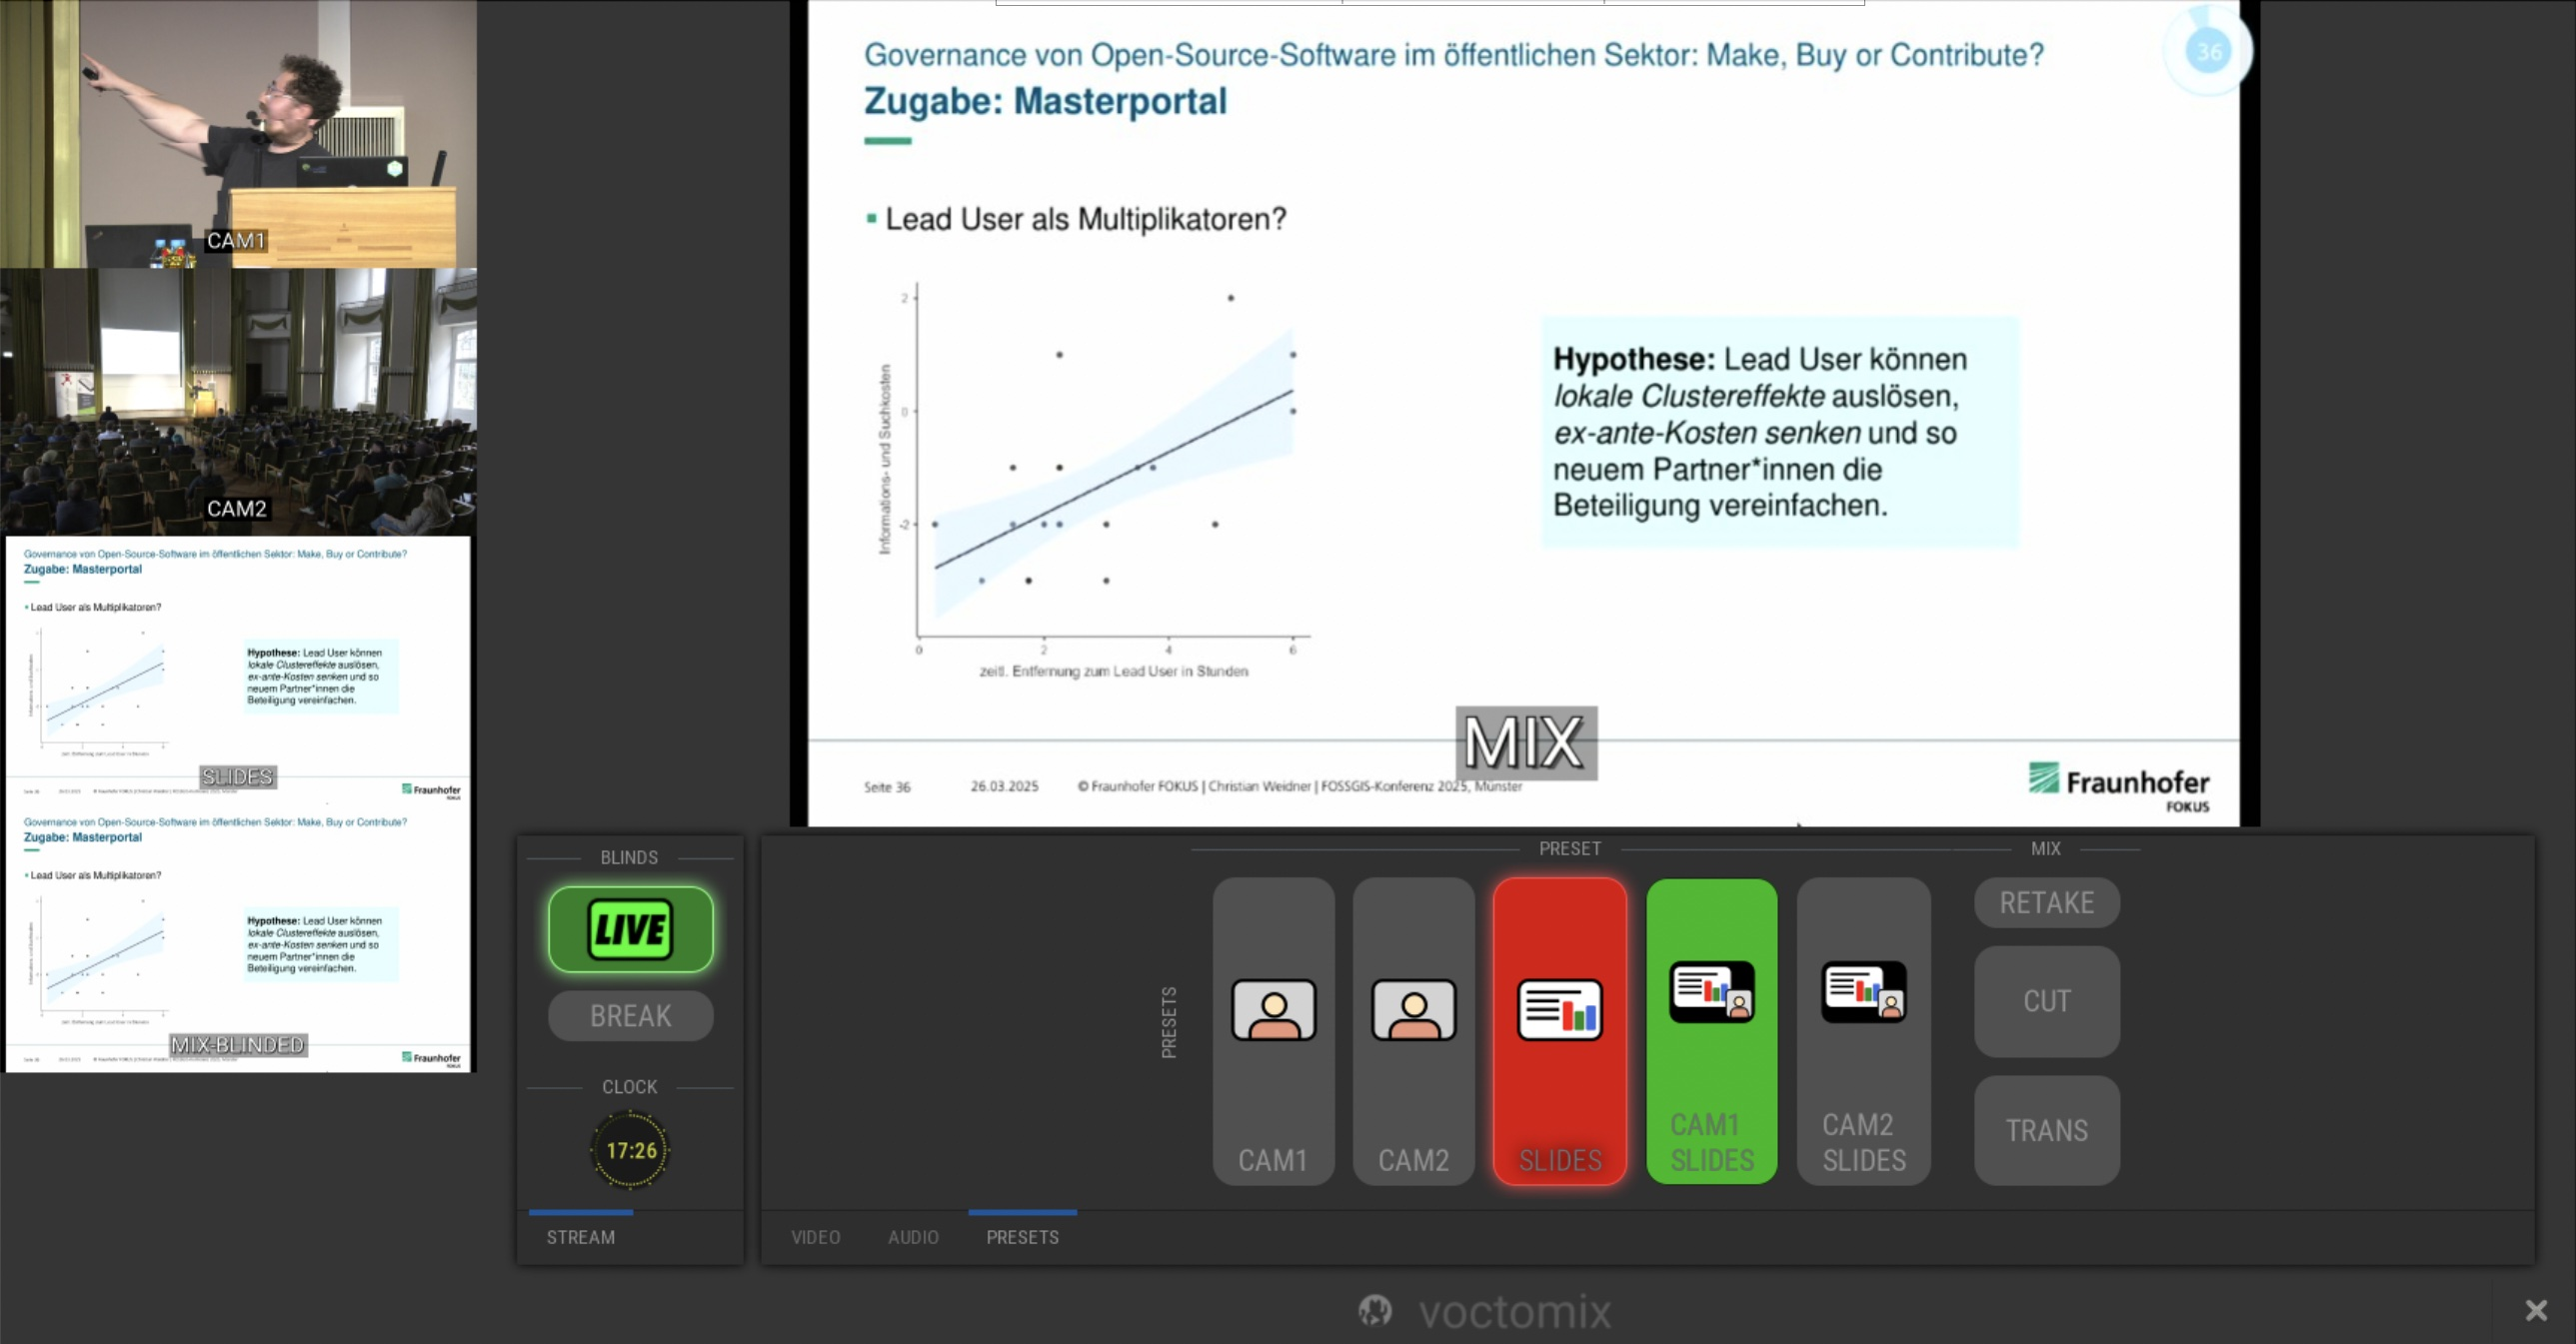
\includegraphics[width=0.9\textwidth]{images/voctomix2-presets-slides.jpg}
		\caption{Voctomix2 Presets: Slides Fullscreen}
	\end{figure}
\end{frame}

%% !TEX root = ../main.tex

\begin{frame}{Telephone}
	\begin{columns}[T,onlytextwidth]
		\column{0.5\textwidth}
		\begin{figure}
			\centering
			\includegraphics[width=0.5\textwidth]{images/telephone.png}
			\caption{Telephone on Mixer Desk}
		\end{figure}
		\column{0.5\textwidth}
		\begin{itemize}
		\item If there are any issues, contact us via Telephone. Just press the VOC Button (red arrow)
		\item Call us via DECT 1601 and state the lecture hall you are in.
		\end{itemize}

	\end{columns}
\end{frame}

\begin{frame}{Intercom: Mixer}
	\begin{columns}[T,onlytextwidth]
		\column{0.5\textwidth}
		\begin{figure}
			\centering
			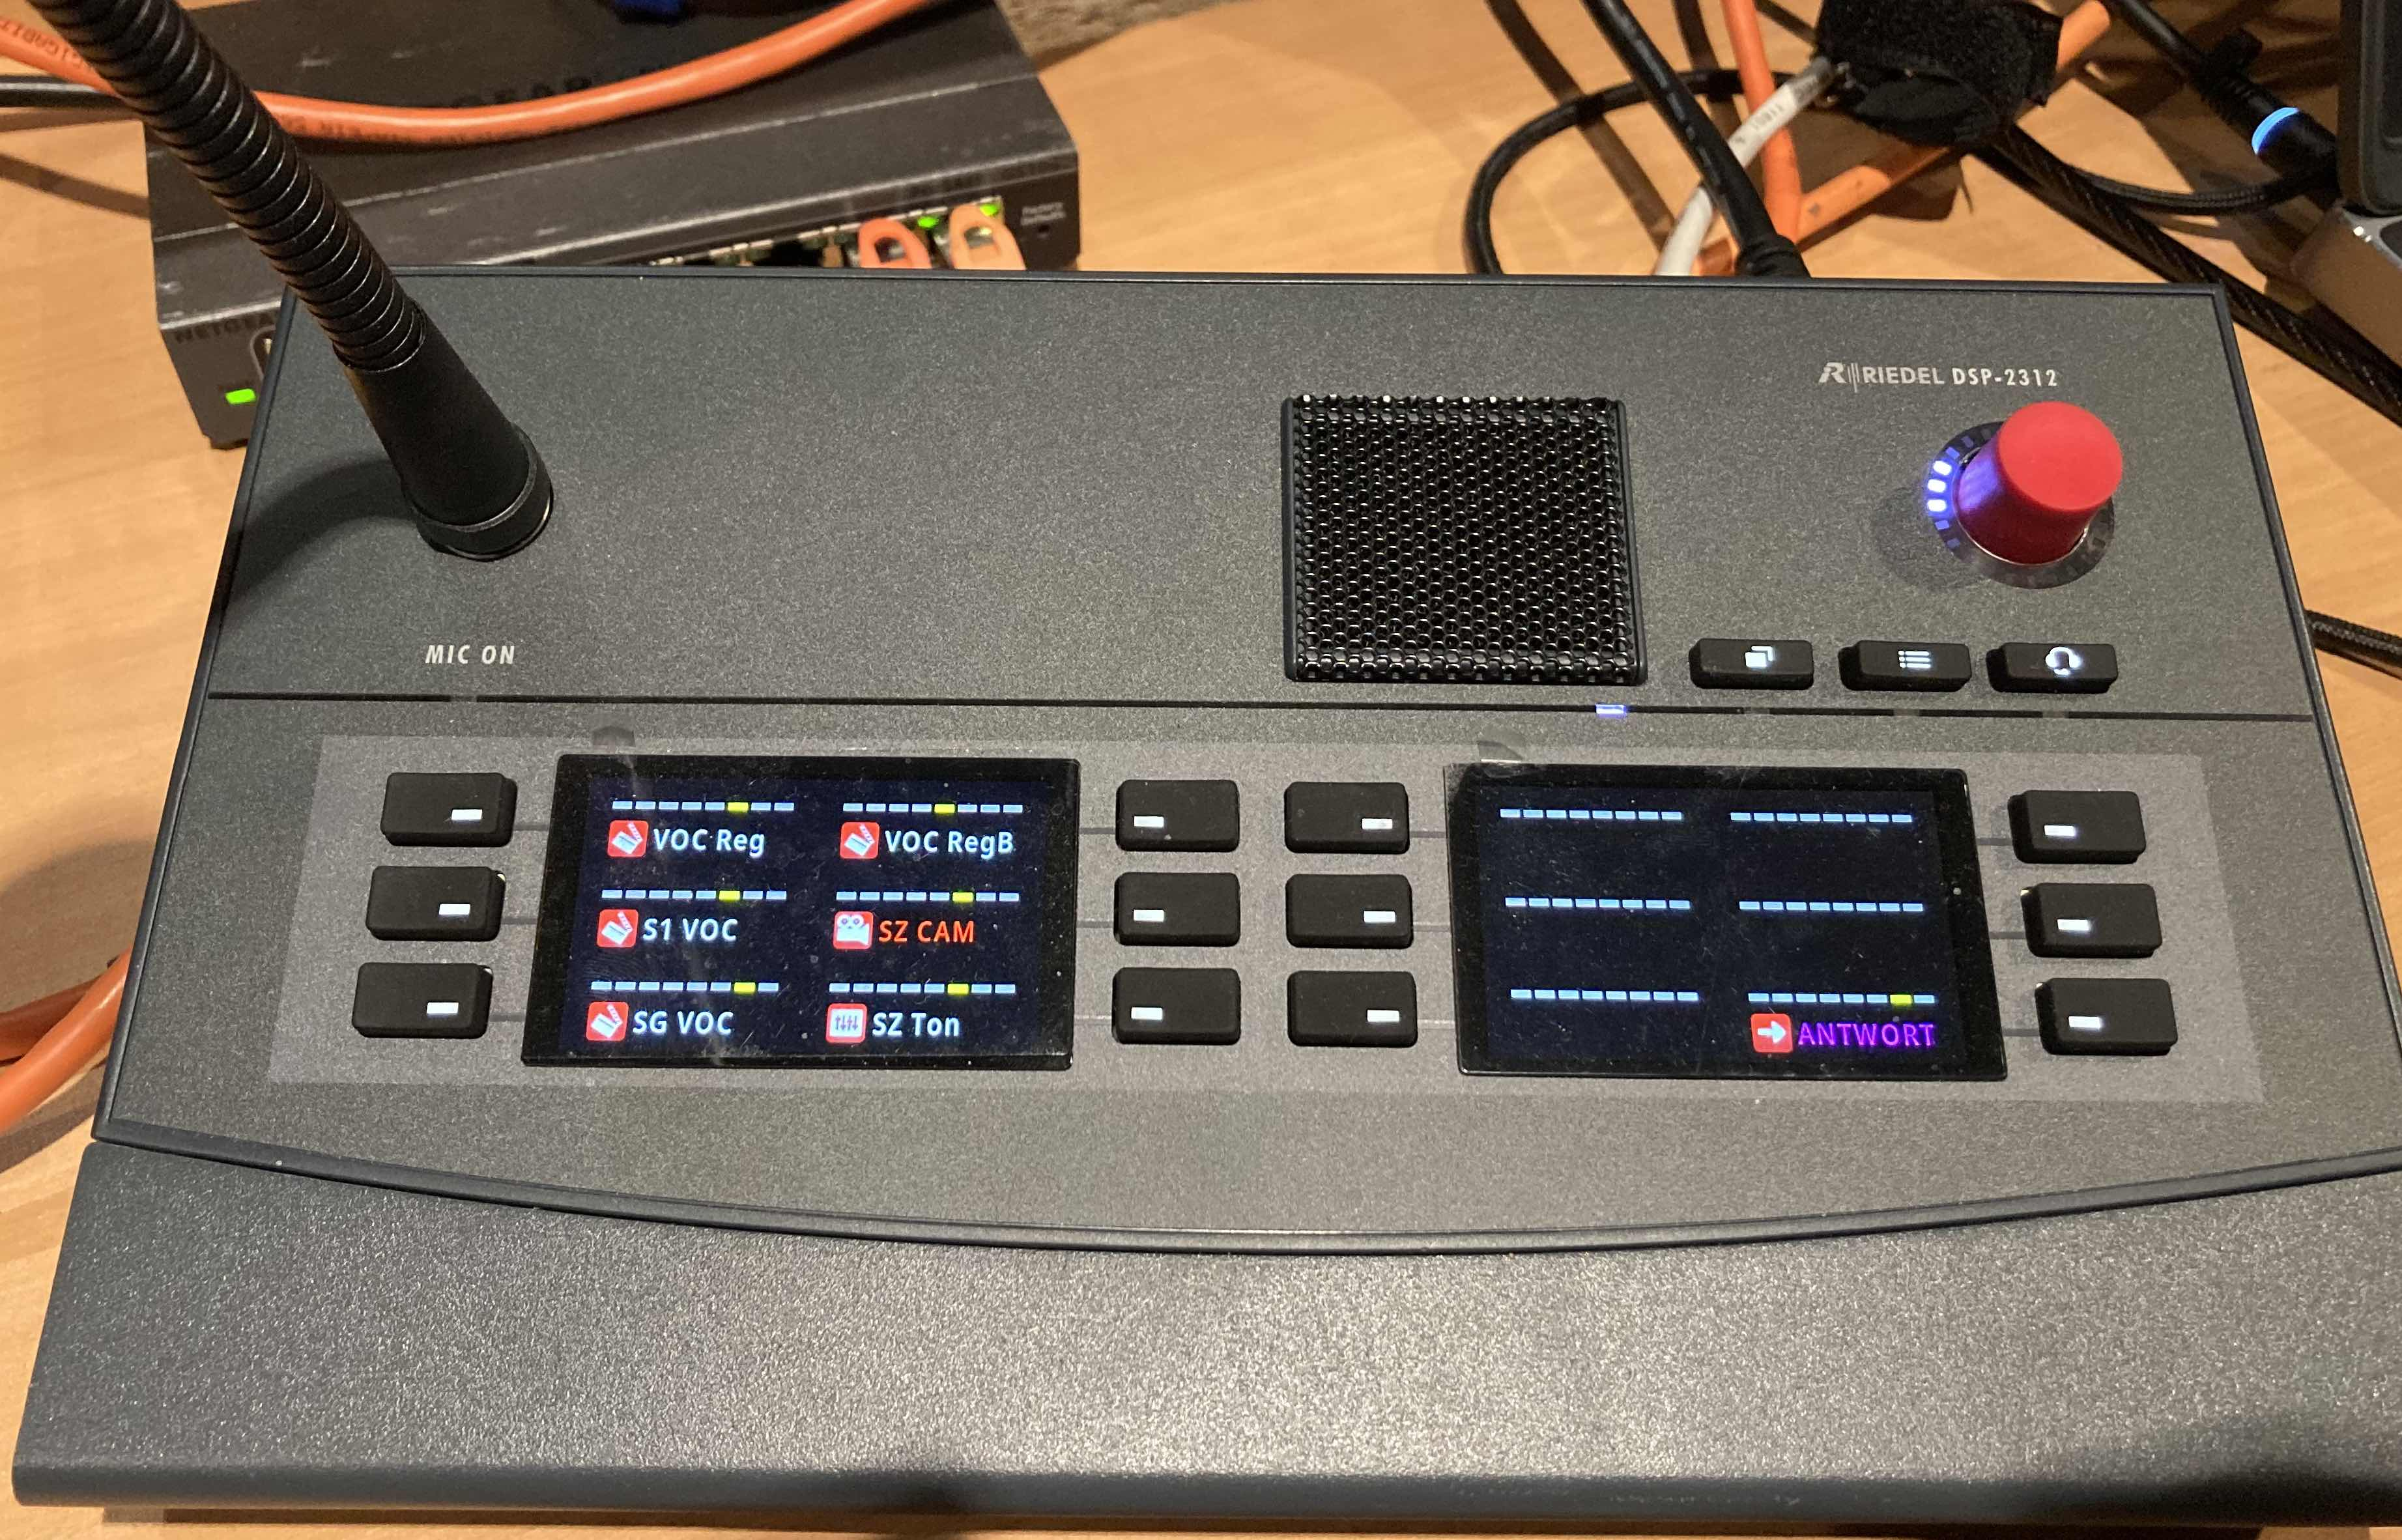
\includegraphics[width=0.9\textwidth]{images/riedel-intercom-panel.jpg}
			\caption{Intercom Device: Main Station}
		\end{figure}
		\column{0.5\textwidth}
			We use a party-line style intercom for communication between mixer and camera
		\begin{itemize}
			\item Press the button next to "CAM" to talk to cameras
			\item Touch channel and turn red knob to adjust volume
		\end{itemize}
	\end{columns}
\end{frame}

\begin{frame}{Intercom: Camera}
	\begin{columns}[T,onlytextwidth]
		\column{0.5\textwidth}
		\begin{figure}
			\centering
			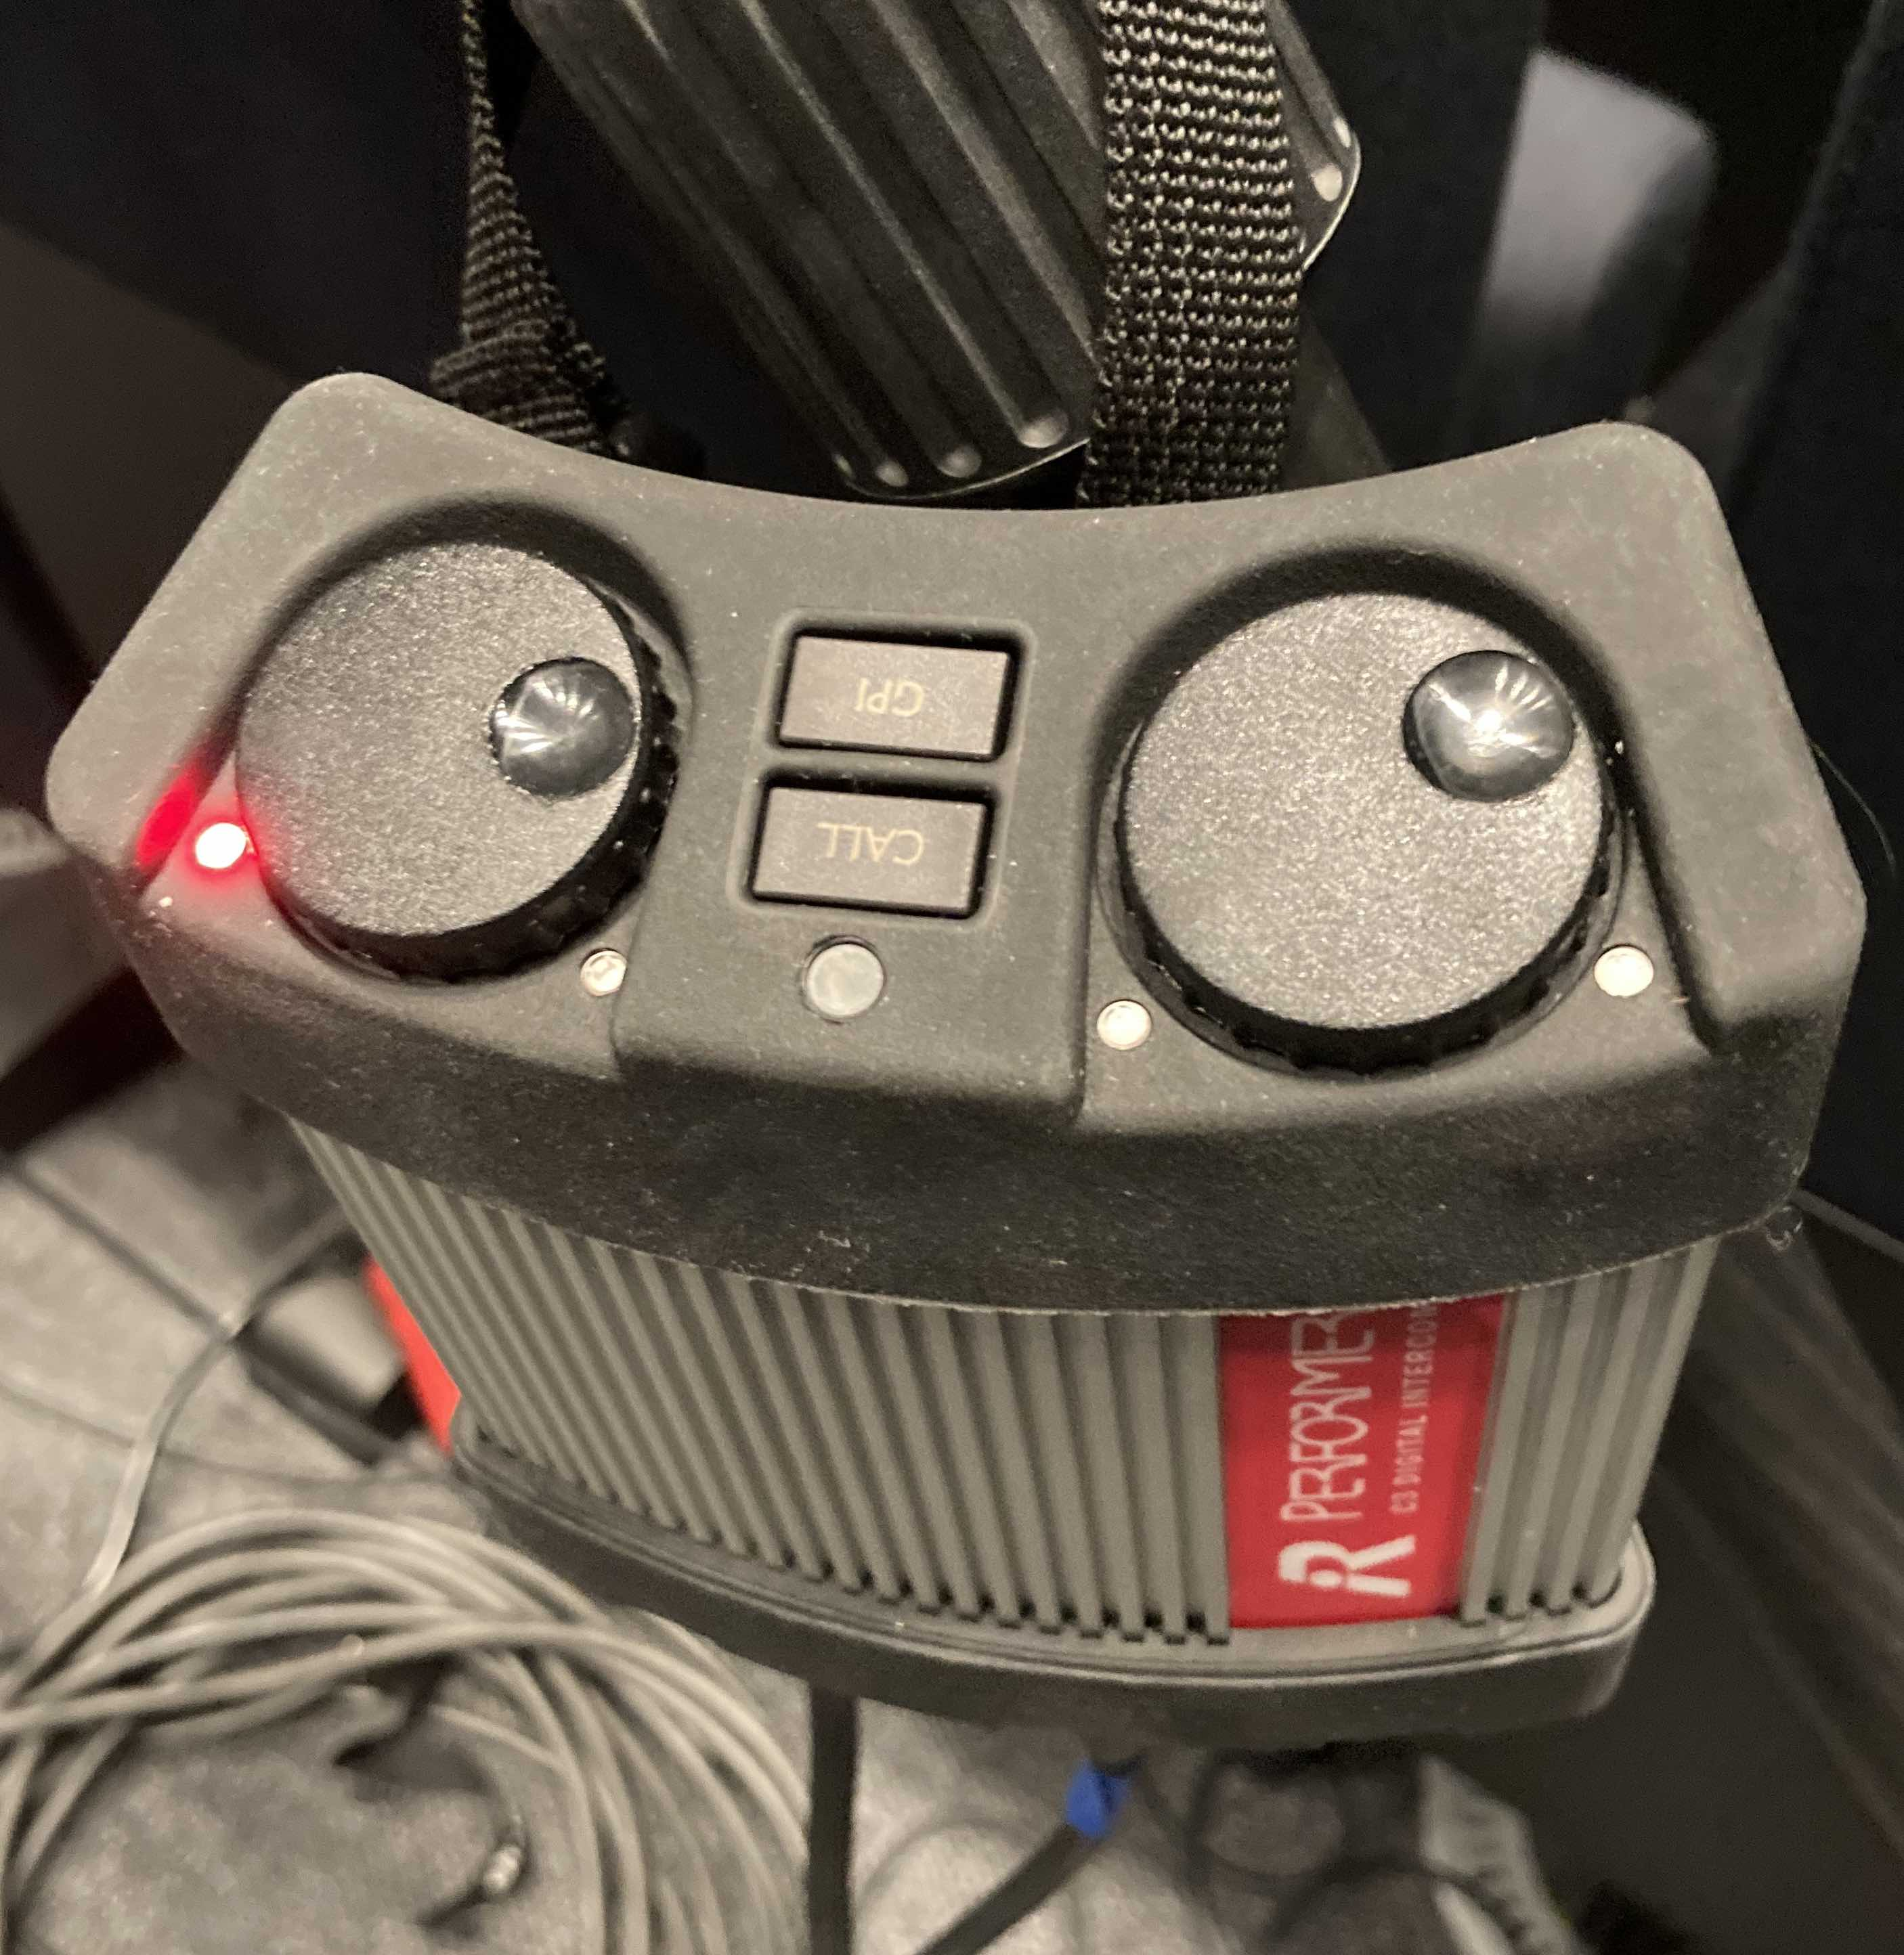
\includegraphics[width=0.75\textwidth]{images/riedel-intercom-artist.jpg}
			\caption{Intercom Device: Camera Station}
		\end{figure}
		\column{0.5\textwidth}

		\begin{itemize}
			\item Press right button to talk
			\item Turn knob to adjust headphone volume
			\item Red light is an inactive channel!
		\end{itemize}
	\end{columns}
\end{frame}

%% !TEX root = ../main.tex

\begin{frame}{Additional Hints}
	\begin{itemize}
		\item Please prefer lecture mode over side-by-side
		\item Don't use side-by-side with two cameras!
		\item Use the intercom to coordinate
		\begin{itemize}
			\item Video mixer should tell when a camera goes on-air
			\item Remind cameras to stay close with the close-up shot
			\item Cameras can request a break
		\end{itemize}
		% \item
	\end{itemize}
\end{frame}



\section{Contacts and Action Items}
\input{chapters/contact-general.tex}
%\input{chapters/contact-congress.tex}
%% !TEX root = ../main.tex

\begin{frame}{Daily Video Mixer Shift Distribution}
	\begin{itemize}
		\item Video mixer shifts are distributed \textbf{every day at 18:00 in Hall 6}
		% \item If you can, you should attend to this meeting.
		% \item We'll distribute information and news there, e.g. if there are any special talks with additional requirements.
		\item Also this meeting should give you the chance of giving each other feedback, ask questions or rise issues.
	\end{itemize}
\end{frame}


\begin{frame}{Final Notes}
	\begin{itemize}
		\item Click "join" on the angel types you want to have
		\item We will approve all known faces/ nick names now
		\item New people will be approved after a shadow shift
		\item Select shifts:
		\begin{itemize}
			\item Fill talks with no angels first
			\item Take breaks
		\end{itemize}
	\end{itemize}
\end{frame}

\end{document}
